% C_exp_1

To find out what happens when words are used in a context where their potential for vagueness comes to the fore, Experiment 1 used three arrays (rather than two) so that the vague description had more than one possible referent, and used indefinite articles to avoid the impression that only one response counted as correct, and was carried out without error feedback. An indication that the potential for vagueness was indeed realised in Experiment 1 is that the borderline response was chosen fairly often: 16\% of the time.

In Experiment 1, an item was an instruction followed by a set of three dot arrays defined by a triple of numbers, representing the number of dots in the left, middle, and right arrays. We used four different triples of numbers: (6,15,24); (16,25,34); (26,35,44); (36,45,54). Each set of arrays comprised three arrays (instead of two as in \citet{green2013utility}); the array representing the central number was always presented in the middle of the three; there were two flanking arrays where one had fewer dots than the central array and the other had more, and these flanking arrays appeared equally often on the left and right of the central array. 

Table \ref{instructionsC-exp-1} gives the full set of stimuli and associated instructions. The way in which borderline responses were construed is as follows, using as an example the array (6:15:24) and instructions that identified the smaller flanking array (6). 6 was classified as the expected response. 15 was classified as the borderline response. 24 was classified as the extreme response. 

\begin{itemize}
	\item In the vague numerical condition the instruction was ``Choose a square with about 10 dots" -- none of the arrays contained exactly 10 dots, but 10 is closer to 6 than it is to 15, making 6 a better response to that instruction, 15 a borderline response, and 24 an extreme response. 
	\item In the vague verbal condition we used ``Choose a square with few dots". We considered this to be equivalent in terms of which responses were expected (6), borderline (15) and extreme (24).
	\item In the crisp numerical condition we used ``Choose the square with 6 dots". The smaller flanking array always contained exactly the specified number of dots. We considered this to be equivalent in terms of which responses were expected (6), borderline (15) and extreme (24).
	\item For crisp verbal, we used ``Choose the square with the fewest dots". We considered this to be equivalent in terms of which responses were expected (6), borderline (15) and extreme (24).
\end{itemize}

On each trial, first the referring expression that constituted the instruction for that trial was displayed (e.g., ``Choose a square with about 10 dots"). Participants then pressed a key to indicate that they had read the instruction. The instruction remained on screen, and after 1000 ms, the arrays appeared. An example stimulus is given in Figure \ref{Experiment1and2examplestimulus}. Response time was measured from the presentation of the arrays until the keypress indicating the participant's choice. The trial would timeout after 60 seconds if there was no response. In this experiment, no feedback was given. This was because, in the vague conditions, we did not regard any response as ``correct" or ``incorrect", but instead as ``expected response"; ``borderline response"; and ``extreme response", and we did not want to draw participants' attention to this distinction explicitly. Which choice the participant made was recorded for analysis.

\begin{table}[htbp]
\centering
\caption{Experiment 1 instructions arranged by condition. The instructions given in the table started with ``Choose \ldots"}
\label{instructionsC-exp-1}
\begin{tabular}{cccll}
\hline\noalign{\smallskip}
Item & Quantity & Number & Crisp & Vague\\
\noalign{\smallskip}\hline\noalign{\smallskip}
06:15:24 & Small & Numeric & the square with 6 dots & a square with about 10 dots\\
06:15:24 & Small & Verbal & the square with the fewest dots & a square with few dots\\
06:15:24 & Large & Numeric & the square with 24 dots & a square with about 20 dots\\
06:15:24 & Large & Verbal & the square with the most dots & a square with many dots\\
\noalign{\smallskip}\hline\noalign{\smallskip}
16:25:34 & Small & Numeric & the square with 16 dots & a square with about 20 dots\\
16:25:34 & Small & Verbal & the square with the fewest dots & a square with few dots\\
16:25:34 & Large & Numeric & the square with 34 dots & a square with about 30 dots\\
16:25:34 & Large & Verbal & the square with the most dots & a square with many dots\\
\noalign{\smallskip}\hline\noalign{\smallskip}
26:35:44 & Small & Numeric & the square with 26 dots & a square with about 30 dots\\
26:35:44 & Small & Verbal & the square with the fewest dots & a square with few dots\\
26:35:44 & Large & Numeric & the square with 44 dots & a square with about 40 dots\\
26:35:44 & Large & Verbal & the square with the most dots & a square with many dots\\
\noalign{\smallskip}\hline\noalign{\smallskip}
36:45:54 & Small & Numeric & the square with 36 dots & a square with about 40 dots\\
36:45:54 & Small & Verbal & the square with the fewest dots & a square with few dots\\
36:45:54 & Large & Numeric & the square with 54 dots & a square with about 50 dots\\
36:45:54 & Large & Verbal & the square with the most dots & a square with many dots\\
\noalign{\smallskip}\hline
\end{tabular}
\end{table}

\begin{figure}[htbp]
\centering
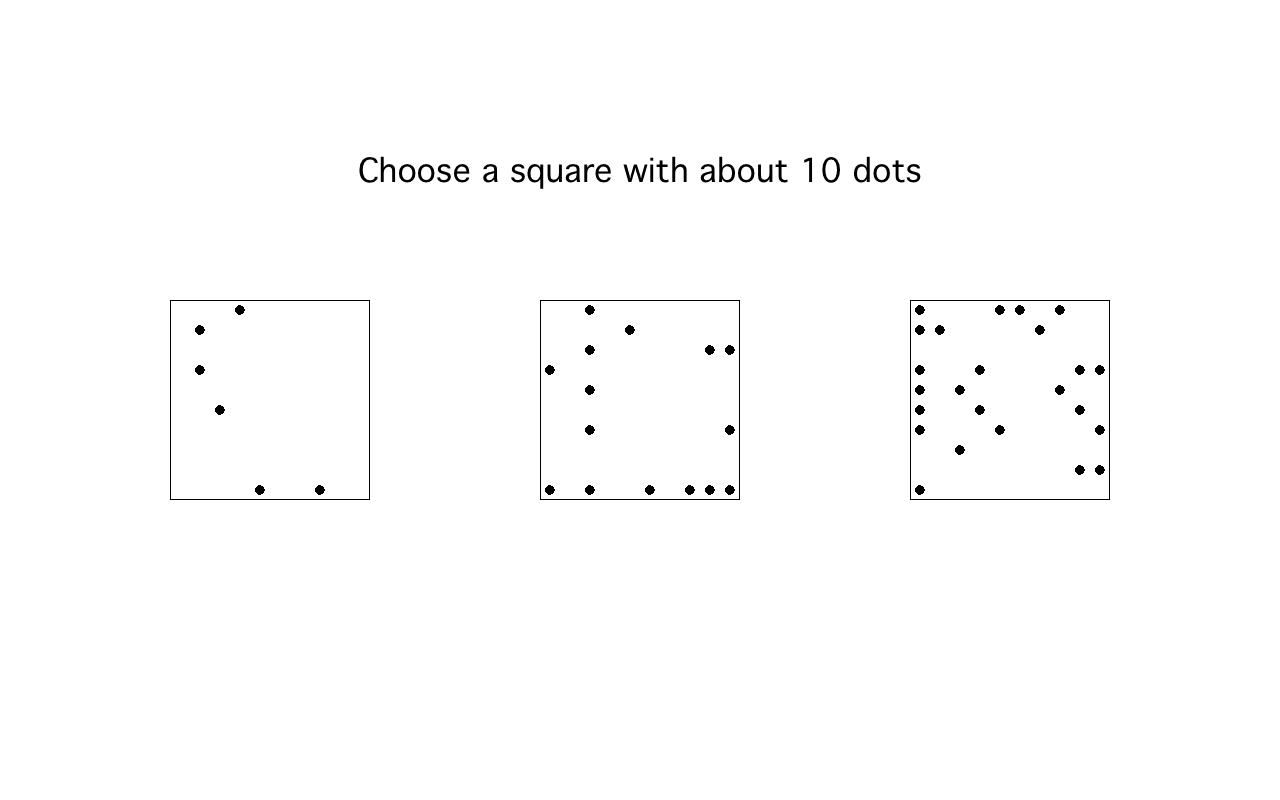
\includegraphics[width=.75\textwidth]{figures/Ce1-example-screenshot}
\caption{Experiment 1 and 2 example stimulus}
\label{Experiment1and2examplestimulus}
\end{figure}

\subsection{Hypotheses (Experiment 1)} 

We formulated the following hypotheses for Experiment 1:

\begin{description}
	\item [Hypothesis 1 (Crisp/Vague RT)] Vague instructions should result in faster responses than crisp instructions; and this pattern should hold when the model is restricted to numeric-only data and when it is restricted to verbal-only data.
	\item [Hypothesis 2 (Numeric/Verbal RT)] There should be no real difference between responses to Numeric instructions and Verbal instructions (based on our interpretation of the experiment in \citet{green2013utility}, where we thought that vague instructions alone were driving the advantage for instructions that were both vague, and also in verbal format).
	\item [Hypothesis 3 (Item RT)] Responses should take longer as the number of dots in the display grows larger (i.e., as the levels of Item increase).
	\item [Hypothesis 4 (Response Type)] Vague instructions should lead to more borderline responses than crisp instructions.
\end{description}

\subsection{Results (Experiment 1)} 

\paragraph{\textbf{Response times}}

30 participants were recruited. Response times from all trials were trimmed at 2.5 standard deviations for each subject, leading to the loss of 236 trials, 3.1\% of the data. The distribution of remaining response times was skewed with many long responses. These remaining response times were log-transformed which reduced this skew so that their distribution more closely approximated a normal distribution. Condition means for response times are given in Figure \ref{resultsC-exp-1-RT}. 

\begin{figure}[htbp]
\centering
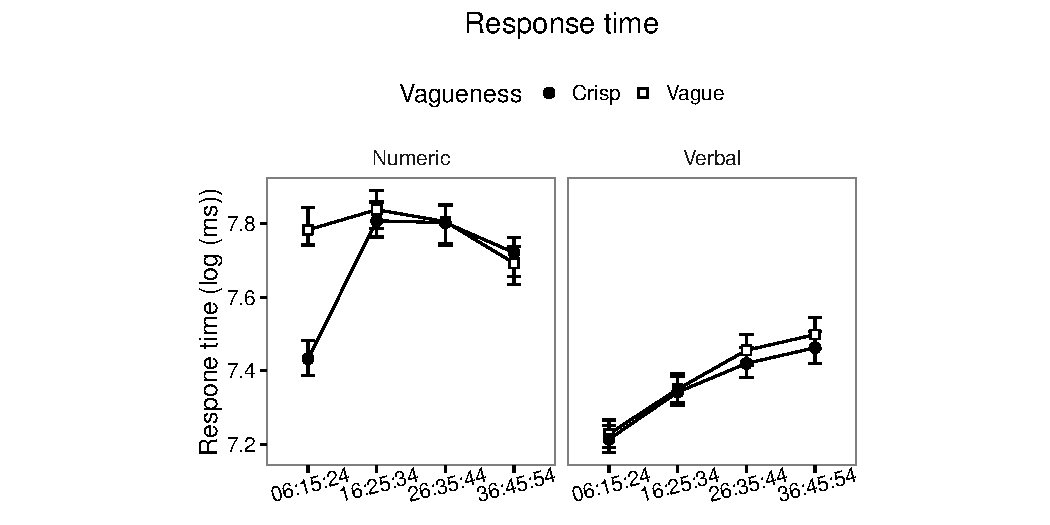
\includegraphics[width=\textwidth]{figures/Ce1-rtplot-1.pdf}
\caption{Experiment 1 results: mean response times by condition and item}
\label{resultsC-exp-1-RT}
\end{figure}

A linear mixed model was constructed for the (log-transformed) response times, with sum-coded vagueness, instruction format, and their interaction, and item, as fixed effects, and per-participant intercepts and slopes for sum-coded vagueness, instruction format, and their interaction as random effects. 

\begin{description}
	\item [Test of Hypothesis 1 (Crisp/Vague RT)] Vague instructions actually led to significantly slower responses than crisp instructions, against Hypothesis 1: $\beta=0.058$, $se=0.013$, $t=4.55$, $p<0.001$. When the model was restricted to numeric-only instructions Vague instructions still led to significantly slower responses than crisp instructions $\beta=0.093$, $se=0.021$, $t=4.51$, $p<0.001$. When the model was restricted to verbal-only instructions Vague instructions tended to slow responses, but not significantly: $\beta=0.024$, $se=0.016$, $t=1.46$, $p=0.155$.
	\item [Test of Hypothesis 2 (Numeric/Verbal RT)] There was actually a significant difference between numeric and verbal instructions, with numeric instructions leading to longer responses than verbal instructions, against Hypothesis 2: $\beta0.265=$, $se=0.072$, $t=5.08$, $p<0.001$.
	\item [Test of Hypothesis 3 (Item RT)] Responses took longer as the levels of Item increased, supporting Hypothesis 3: $\beta=0.120$, $se=0.017$, $t=7.11$, $p<0.001$.
\end{description}

However, given that the response time plot in Figure \ref{resultsC-exp-1-RT} shows that responses to 6:15:24 in the "crisp numeric" instructions condition were extremely fast relative to the "vague numeric" instructions to 6:15:24, the effects in the model of the full dataset could be driven by this difference. A clearer picture of the effects of interest might be obtained by removing the 6:15:24 level of Item from the data set, and fitting the model to this restricted data. Doing this did not affect the direction of the effects in the full dataset, but whereas the effects were significant in the full dataset, they were not significant in the restricted dataset. Full details of the analysis of the restricted dataset are available in the online materials.

\paragraph{\textbf{Borderline cases}}

A generalized linear mixed model \citet{jaeger2008categorical} was fit to the data for the distribution of responses indicating the borderline response, with sum-coded vagueness, instruction format, (and their interaction), and item as fixed effects, and the same effects as slopes over participant, as well as per-participant intercepts as random effects. The distribution of responses over the nearest match square, the borderline square, and the furthest match square are given in Figure \ref{resultsC-exp-1-BL}. Participants chose the borderline square on $16.6\%$ of trials overall.

\begin{figure}[htbp]
\centering
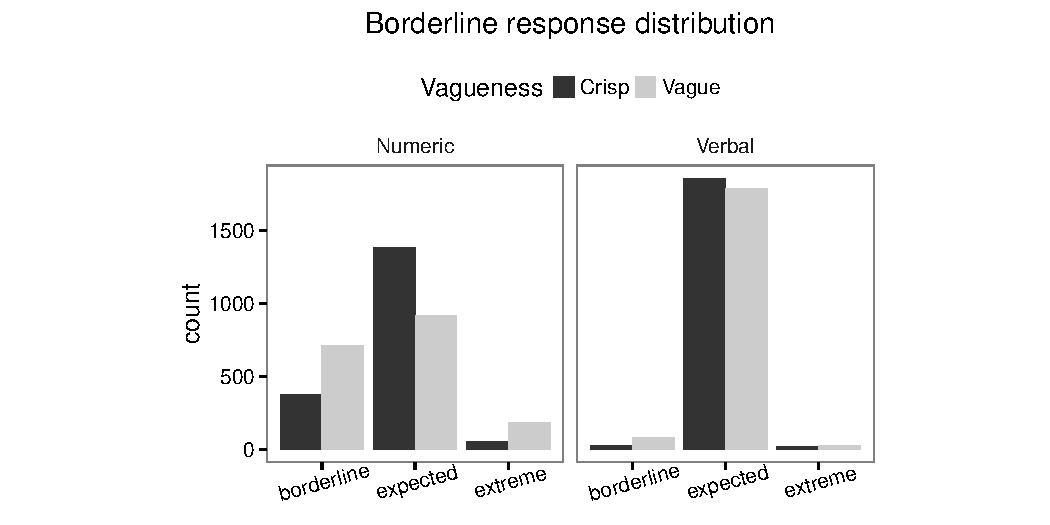
\includegraphics[width=\textwidth]{figures/Ce1-blBarChart-1}
\caption{Experiment 1 results: counts of borderline case responses by condition.}
\label{resultsC-exp-1-BL}
\end{figure}

\begin{description}
	\item [Test of Hypothesis 4 (Response Type)] Participants were significantly more likely to choose the borderline option for vague instructions than for crisp instructions (21.9\% vs 11.3\%: $\beta=0.62$, $se=0.22$, $z=2.8$, $p=0.0059$). Participants were also significantly more likely to choose the borderline square when the instruction used the numerical format rather than the verbal format (30.1\% vs 3.0\%: $\beta=-3.35$, $se=0.23$, $z=-14.6$, $p<0.0001$). 
\end{description}

\subsection{Discussion (Experiment 1)}

This experiment tested whether vague instructions would result in faster responses than crisp instructions, when borderline cases were present. Faster responses for vague instructions were found in pilot experiment B, but there were no borderline cases in that experiment.

In this experiment we found in contrast that vague instructions resulted in slower responses than crisp instructions: a difference that was significant when considering the full data (112ms), but which was not significant after removing the smallest arrays from the analysis, which had a pattern opposite to the main trends in the rest of the data.

We also found that the effect of instruction format was significant, with numerical format slowing responses by 689 ms on average, such that the disadvantage of numerical format overwhelmed the contribution of vagueness. The verbal vague condition still yielded faster responses than the numerical crisp condition, so the pattern from pilot experiment B was reproduced, but in the light of the evidence from this experiment (Experiment 1), in the presence of borderline cases, the advantage that was ascribed to vagueness before now looks more like an advantage of verbal instruction format.

However, once again there is a possibly confounding factor. Observe that, in Experiment 1, instruction format (i.e., the difference between numeric and verbal) went hand in hand with might be called the (human) "selection algorithm": To see this, consider the task of selecting the dot array that contains "few dots":" to do this, it suffices to \emph{compare} the three arrays and select the one that contains the fewest elements.  To select the dot array that contains "16 dots" seems to require the participant to estimate, and then \emph{match}, the cardinality of (at least) one dot array to 16, a process which could plausibly take longer, independently of vagueness. Therefore, our results so far permit the interpretation that what made the instructions in the verbal condition fast is not the fact that they were worded verbally, but that they allowed participants to use \emph{comparison} rather than having to resort to \emph{matching}.

In the next two experiments we pitted the comparison algorithm and matching algorithm selection tasks against each other while controlling vagueness and instruction format. In Experiment 2 we restricted all the instructions to numeric quantifiers while factorially manipulating vagueness and selection task. In Experiment 3 we ensured that all instructions used verbal quantifiers, while also factorially manipulating vagueness and selection task. This allowed us to distinguish between the predictions of the selection task account and the instruction format account. 
